\documentclass[12pt, a4paper]{article}

% --- MAIN PACKAGES ---
\usepackage[utf8]{inputenc}
\usepackage[T1]{fontenc}
\usepackage{lmodern}
\usepackage[english]{babel}
\usepackage{amsmath, amssymb}
\usepackage{graphicx}
\usepackage{booktabs}
\usepackage{array}
\usepackage{listings}
\usepackage{xcolor}
\usepackage{tikz}
\usetikzlibrary{positioning, arrows.meta}
\usepackage[margin=2.5cm]{geometry}
\usepackage{hyperref}

% Python code style
\definecolor{codegreen}{rgb}{0,0.6,0}
\definecolor{codegray}{rgb}{0.5,0.5,0.5}
\definecolor{codepurple}{rgb}{0.58,0,0.82}
\definecolor{backcolour}{rgb}{0.96,0.96,0.96}

\lstdefinestyle{mystyle}{
    backgroundcolor=\color{backcolour},
    commentstyle=\color{codegreen},
    keywordstyle=\color{magenta},
    numberstyle=\tiny\color{codegray},
    stringstyle=\color{codepurple},
    basicstyle=\ttfamily\footnotesize,
    breaklines=true,
    captionpos=b,
    keepspaces=true,
    numbers=left,
    showspaces=false,
    showstringspaces=false,
    showtabs=false,
    tabsize=2
}
\lstset{style=mystyle}

% --- DOCUMENT AND GROUP DATA (5 MEMBERS) ---
\title{\textbf{Technical Documentation: The Random Forest Algorithm}}

\author{
  \begin{tabular}{c}
    Laura Chevarría Saravia \qquad Daniel Betancor Andueza \\
    Álvaro Ginés Gómez \qquad Sergio Alejandro Medina Ospina \\
    Yousef Ahmed Kassem
  \end{tabular} \\[0.3cm]
  \small Degree in Data Science and Engineering --- Professional Skills for Engineers (HPI) \\
  \small University of Las Palmas de Gran Canaria (ULPGC)
}

\date{\today}

\begin{document}

\maketitle

\begin{abstract}
This document provides a self-contained technical description of the supervised learning algorithm \textit{Random Forest}. It analyses the overfitting problem of single decision trees, variance reduction through bootstrap aggregation (\textit{bagging}) and tree decorrelation through random feature selection at each node. The Gini impurity is developed with a complete numerical example, the proportion of \textit{Out-Of-Bag} (OOB) data is derived, and we show why averaging weakly correlated trees reduces variance. The document includes a diagram of the algorithm's workflow, a comparison table and a short Python implementation using \texttt{scikit-learn}.
\end{abstract}

\section{Introduction}
Single decision trees (CART) are intuitive, non-parametric models; however, they have high variance and a strong tendency to overfit: small changes in the training data produce very different trees. The \textit{Random Forest} algorithm, proposed by Leo Breiman~\cite{breiman2001}, reduces this limitation through an \textit{ensemble learning} approach: it combines many trees trained independently on resampled versions of the data and aggregates their predictions, in both classification and regression~\cite{salman2024}.

\section{Notation}
We start from a training set $D$ with $N$ observations and $M$ features, arranged as a design matrix $\mathbf{X}$ and a label vector $\mathbf{y}$:
\begin{equation}
\mathbf{X} =
\begin{bmatrix}
x_{11} & x_{12} & \cdots & x_{1M} \\
x_{21} & x_{22} & \cdots & x_{2M} \\
\vdots & \vdots & \ddots & \vdots \\
x_{N1} & x_{N2} & \cdots & x_{NM}
\end{bmatrix} \in \mathbb{R}^{N \times M},
\qquad
\mathbf{y} =
\begin{bmatrix}
y_1 \\ y_2 \\ \vdots \\ y_N
\end{bmatrix}.
\end{equation}
Each row $\mathbf{x}_i$ is an observation and each column a feature. The forest consists of $B$ trees $T_1, \dots, T_B$.

\section{Mathematical Foundations}

\subsection{Gini Impurity Criterion}
To build each node of a tree, the algorithm looks for the feature and threshold that make the resulting subsets as \emph{pure} as possible, that is, with a clear majority of a single class. The Gini impurity $G$ of a node is defined as:
\begin{equation}
G = 1 - \sum_{k=1}^{K} p_k^2
\label{eq:gini}
\end{equation}
where $K$ is the number of classes and $p_k$ is the proportion of observations of class $k$ in the node. A pure node has $G=0$; with two classes at 50\,\% each, the maximum $G=0.5$ is reached.

If a parent node with $n$ observations is split into a left child ($n_L$) and a right child ($n_R$), the quality of the split is measured by the \emph{impurity decrease}:
\begin{equation}
\Delta G = G_{\text{parent}} - \left( \frac{n_L}{n}\, G_L + \frac{n_R}{n}\, G_R \right)
\label{eq:deltagini}
\end{equation}
and the split with the largest $\Delta G$ is chosen.

\subsection{Bagging and Random Subspaces}
Training combines \textit{bagging} (\textit{Bootstrap Aggregating})~\cite{amara2024} with random feature selection, in three steps:
\begin{enumerate}
    \item $B$ bootstrap samples $D_1,\dots,D_B$ are drawn, each containing $N$ observations chosen \emph{with replacement} from $D$.
    \item A tree $T_b$ is trained on each $D_b$. At each node, only $m \le M$ randomly chosen features are considered (typically $m = \sqrt{M}$ for classification and $m = M/3$ for regression).
    \item For a new observation $\mathbf{x}$, the predictions of the trees are aggregated:
\end{enumerate}
\begin{equation}
\hat{Y}(\mathbf{x}) =
\begin{cases}
\operatorname{mode}\left\{ T_1(\mathbf{x}), \dots, T_B(\mathbf{x}) \right\}, & \text{for classification (majority vote)},\\[6pt]
\dfrac{1}{B} \displaystyle\sum_{b=1}^{B} T_b(\mathbf{x}), & \text{for regression (average)}.
\end{cases}
\label{eq:aggregation}
\end{equation}

\subsection{Why Does It Work? Variance Reduction}
Assume each tree has variance $\sigma^2$ and that the correlation between any two trees is $\rho$. The variance of the average of the $B$ trees is:
\begin{equation}
\operatorname{Var}\!\left( \frac{1}{B} \sum_{b=1}^{B} T_b(\mathbf{x}) \right)
= \rho\,\sigma^2 + \frac{1-\rho}{B}\,\sigma^2 .
\label{eq:variance}
\end{equation}
The second term vanishes as $B$ grows, but the first does not: if the trees are highly correlated ($\rho \approx 1$), adding more trees barely helps. This is why \textit{Random Forest} draws $m$ random features at each node: it forces the trees to differ, lowering $\rho$ and therefore the total variance. This is the difference from plain bagging, which only resamples observations.

\subsection{Out-Of-Bag (OOB) Error Estimation}
When sampling with replacement, a given observation is not picked in a single draw with probability $1 - \frac{1}{N}$. Since $N$ independent draws are made, the probability that it is left out of the bootstrap sample is:
\begin{equation}
P(\text{not in } D_b) = \left(1 - \frac{1}{N}\right)^{N}
\xrightarrow[N \to \infty]{} e^{-1} \approx 0.368 .
\label{eq:oob}
\end{equation}
For example, with $N=10$ we already get $0.9^{10} \approx 0.349$. Thus, each tree leaves out about 36.8\,\% of the data (the \textit{Out-Of-Bag} observations). By predicting each observation only with the trees that did not see it, we obtain an internal estimate of the generalisation error without setting aside a separate validation set~\cite{salman2024}.

\section{Worked Example: Choosing the Split}
We use the classroom example from~\cite{cs307}: 10 observations, two binary features $X_1, X_2 \in \{T, F\}$ and a label $Y \in \{+,-\}$, as shown in Table~\ref{tab:data}.

\begin{table}[htbp]
\centering
\caption{Example data (each row appears \textit{Count} times).}
\label{tab:data}
\begin{tabular}{cccc}
\toprule
$X_1$ & $X_2$ & $Y$ & \textbf{Count} \\
\midrule
T & T & $+$ & 2 \\
T & F & $+$ & 2 \\
F & T & $-$ & 5 \\
F & F & $+$ & 1 \\
\bottomrule
\end{tabular}
\end{table}

\paragraph{Step 1: impurity of the root node.} There are 5 positives and 5 negatives, so by~\eqref{eq:gini}:
\[
G_{\text{root}} = 1 - \left(\tfrac{5}{10}\right)^2 - \left(\tfrac{5}{10}\right)^2 = 0.5 .
\]

\paragraph{Step 2: splitting on $X_1$.} With $X_1 = T$ there are 4 observations, all positive ($G_L = 0$). With $X_1 = F$ there are 6: 1 positive and 5 negative:
\[
G_R = 1 - \left(\tfrac{1}{6}\right)^2 - \left(\tfrac{5}{6}\right)^2 = \tfrac{10}{36} \approx 0.278,
\qquad
\Delta G_{X_1} = 0.5 - \left( \tfrac{4}{10}\cdot 0 + \tfrac{6}{10}\cdot 0.278 \right) \approx 0.333 .
\]

\paragraph{Step 3: splitting on $X_2$.} With $X_2 = T$ there are 7 observations (2 positive, 5 negative); with $X_2 = F$ there are 3, all positive ($G_R = 0$):
\[
G_L = 1 - \left(\tfrac{2}{7}\right)^2 - \left(\tfrac{5}{7}\right)^2 = \tfrac{20}{49} \approx 0.408,
\qquad
\Delta G_{X_2} = 0.5 - \left( \tfrac{7}{10}\cdot 0.408 + \tfrac{3}{10}\cdot 0 \right) \approx 0.214 .
\]

\paragraph{Conclusion.} Since $\Delta G_{X_1} > \Delta G_{X_2}$, the tree splits on $X_1$ first, the same choice given by information gain in~\cite{cs307}. In a \textit{Random Forest} with $m = 1$, each node would draw one of the two features at random, so some trees would start with $X_2$: this is precisely the diversity that lowers $\rho$ in~\eqref{eq:variance}.

\section{Algorithm Structure and Evaluation}

Figure~\ref{fig:rf_flow} illustrates the training and aggregation workflow of the ensemble.

\begin{figure}[!ht]
\centering
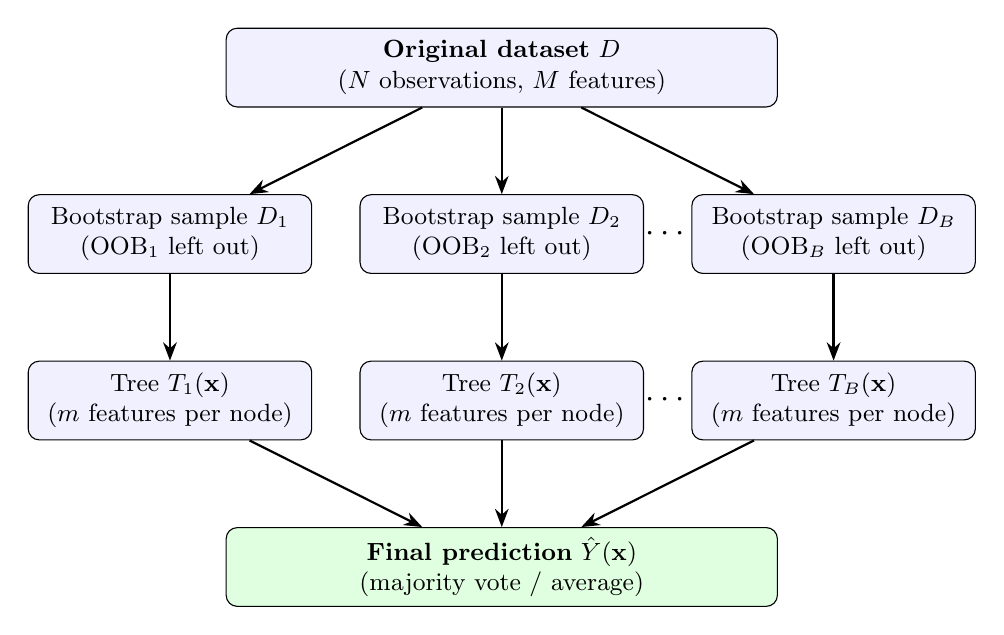
\begin{tikzpicture}[
  box/.style={draw, fill=blue!6, rounded corners, align=center, font=\small,
               minimum width=3.6cm, minimum height=1cm},
  arrow/.style={-{Stealth}, thick},
  node distance=1.1cm and 0.6cm
]
  \node[box, minimum width=7cm] (data) {\textbf{Original dataset} $D$ \\ ($N$ observations, $M$ features)};

  \node[box, below=of data] (b2) {Bootstrap sample $D_2$ \\ (OOB$_2$ left out)};
  \node[box, left=of b2]    (b1) {Bootstrap sample $D_1$ \\ (OOB$_1$ left out)};
  \node[box, right=of b2]   (b3) {Bootstrap sample $D_B$ \\ (OOB$_B$ left out)};

  \node[box, below=of b1] (t1) {Tree $T_1(\mathbf{x})$ \\ ($m$ features per node)};
  \node[box, below=of b2] (t2) {Tree $T_2(\mathbf{x})$ \\ ($m$ features per node)};
  \node[box, below=of b3] (t3) {Tree $T_B(\mathbf{x})$ \\ ($m$ features per node)};

  \node[box, fill=green!12, minimum width=7cm, below=of t2] (agg)
       {\textbf{Final prediction} $\hat{Y}(\mathbf{x})$ \\ (majority vote / average)};

  \path (b2) -- (b3) node[midway, font=\large] {$\cdots$};
  \path (t2) -- (t3) node[midway, font=\large] {$\cdots$};

  \foreach \b/\t in {b1/t1, b2/t2, b3/t3} {
    \draw[arrow] (data) -- (\b);
    \draw[arrow] (\b) -- (\t);
    \draw[arrow] (\t) -- (agg);
  }
\end{tikzpicture}
\caption{Block diagram of the Random Forest architecture.}
\label{fig:rf_flow}
\end{figure}

Table~\ref{tab:rf_vs_cart} summarises the key differences between a single decision tree and the \textit{Random Forest} ensemble.

\begin{table}[htbp]
\centering
\caption{Comparison between a single decision tree and Random Forest.}
\label{tab:rf_vs_cart}
\small
\begin{tabular}{>{\raggedright}p{3.6cm} >{\raggedright}p{5cm} >{\raggedright\arraybackslash}p{5cm}}
\toprule
\textbf{Property} & \textbf{Decision tree (CART)} & \textbf{Random Forest} \\
\midrule
Model variance & High (prone to overfitting) & \textbf{Low} (reduced by aggregating trees) \\
Features per node & Evaluates all $M$ features & Random subset, e.g.\ $m = \sqrt{M}$ \\
Interpretability & High (direct rules) & Moderate (black-box-like) \\
Error estimation & Requires a separate validation set & Internal OOB error \\
Missing data & Sensitive & \textbf{Robust} (proximity matrix) \\
\bottomrule
\end{tabular}
\end{table}

\section{Conclusion}
\textit{Random Forest} is one of the most versatile algorithms in Data Science. Its double randomness (in the observations, through bootstrapping, and in the features considered at each node) decorrelates the individual trees, which, according to~\eqref{eq:variance}, reduces the variance of the ensemble and mitigates the overfitting of a single tree. In addition, the OOB estimate makes it possible to evaluate the model without extra data.

\begin{thebibliography}{9}
\bibitem{breiman2001}
L.~Breiman, ``Random Forests'', \textit{Machine Learning}, vol.~45, no.~1, pp.~5--32, 2001.

\bibitem{salman2024}
H.~A. Salman, A.~Kalakech and A.~Steiti, ``Random Forest Algorithm Overview'', \textit{Babylonian Journal of Machine Learning}, vol.~2024, pp.~69--79, 2024. \url{https://doi.org/10.58496/BJML/2024/007}

\bibitem{amara2024}
Y.~Amara-Ouali, \textit{Random Forests} (session 2 slides), 2024.

\bibitem{cs307}
\textit{CS 307: Random Forests} (lecture slides).
\end{thebibliography}

\end{document}